\documentclass{article}
\usepackage[utf8]{inputenc}
\usepackage{amsmath}
%\usepackage[norsk]{babel}
\usepackage{amssymb}
\usepackage{tikz}
\usetikzlibrary{decorations.markings}
\usepackage{empheq}
\usepackage{amsthm}
\usepackage{pgfplots}
\usetikzlibrary{decorations.pathreplacing}
\usetikzlibrary{calc}
\usepackage{xcolor}
\usepackage{physics}
\usepackage{fancyhdr}
\pagestyle{fancy}
\usepackage{esdiff}
\usepackage{tikz-feynman}
\usepackage{hyperref}


\title{Lecture notes FY8305}

\date{August, 2019}


\theoremstyle{definition}
\newtheorem{exmp}{Example}[section]



\newcommand{\e}{\mathrm{e}}
%\newcommand{\dd}{\mathrm{d}}


\tikzset{->-/.style={decoration={
  markings,
  mark=at position #1 with {\arrow{>}}},postaction={decorate}}}

\begin{document}

\maketitle
Digitialized from ``FAG 74986 Funksjonal-integral metoder HØST 1996''.
Used as lecture notes for self-study in the course ``FY8305 - Functional Integral Methods in Condensed Matter Physics''. \href{https://www.ntnu.edu/studies/courses/FY8305}{\textbf{Link to course page}}

\tableofcontents

\section{Short recap of second quantization for fermions and bosons}

Notation: $ \mu = $ set of quantum numbers that define a one-particle state.


\subsection{Many particle basis}
\newtheorem{theorem}{Ex}
\begin{theorem}


\begin{align*}
\mu &= (\vec{k}, \sigma):\text{Wave number, spin} \\
\mu &= (i, \sigma) : \text{Lattice point, spin} \\
\mu &= (n, i) : \text{Orbital, lattice point} \\
\end{align*}

\end{theorem}

A many-particle basis can be written $\ket{\phi} = \ket{n_{\mu}, n_{\nu}, \dots, n_{\mu_N}}$. Many particle states are built by combining many one-particle states, but where the one-particle states are not necessarily independent. If  \underline{one} of the set of quantum numbers, $\mu_i$, are changed, this \underline{scattering} will generally have consequences for the distribution of quantum numbers for the remaining sets $\{\mu_j\}_{j\ne i}$.
We generally imagine that many-particle states can be built as a linear combination of
$\ket{\phi}$'s;
\begin{equation}
\ket{\Psi} = \sum_{n_{\mu},\dots, n_{\mu_N}}\phi_{{\mu},\dots, n_{\mu_N}}\ket{{\mu},\dots, n_{\mu_N}}.
\end{equation}
A definite one-state vector $\ket{n_{\mu},\dots, n_{\mu_N}}$ can be demanded from a vacuum state (where there is no filled one-particle states) $\ket{0}$ via creation operators.
\begin{align*}
&\textbf{bosons}: &a_\mu^\dagger \\ 
&\textbf{fermions}: &c_\mu^\dagger
\end{align*}


A quanta in a one-particle state can be destroyed by the annihilation operators.

\begin{align*}
&\textbf{bosons}: &a_\mu \\ 
&\textbf{fermions}: &c_\mu
\end{align*}


These operators satisfy some commutation relations:
\begin{align}
&[a_\mu, a_{\nu}] & = [a_\mu^\dagger, a_{\nu}^\dagger] = 0 \\
&[a_\mu, a_{\nu}^\dagger] & = \delta_{\mu\,\nu} \\
&[A,B] &= AB-BA \\
&\{c_\mu^\dagger, c_{\nu}^\dagger\} & = \{c_\mu, c_{\nu}\} = 0 \\
&\{c_\mu, c_{\nu}^\dagger\} & = \delta_{\mu\,\nu} \\
&\{A,B\} &= AB + BA
\end{align}
These will automatically satisfy the Pauli principle as well, which gives \emph{symmetri/ \emph{antisymmetric}} solutions by exchange, dependent if the particles are bosons/fermions. 


\subsection{From classical formulation to second quantization of one-particle operators}

For one-particle operators we usually have a kinetic energy function on a form like
\begin{equation}
T = \sum_i T\left(\vec{r}_i, \vec{p}_i\right) = \sum_i T\left(\vec{r}_i, \diffp{}{r}\right)
\end{equation}
\begin{theorem}
External electrostatic potential:
\begin{equation}
T = \sum_i V_{\text{ext}}\left(\vec{r}_i\right)
\end{equation}
\end{theorem}
\begin{theorem}

Kinetic energy:

\begin{equation}
T = \sum_i \frac{p^2}{2m} = -\sum_i \frac{\hbar^2}{2m}\nabla_i^2
\end{equation}
\end{theorem}

\begin{theorem}
Crystal-potential:
\begin{equation}
T = \sum_i \sum_j v_{\text{cryst}} \left( \vec{r}_i, \vec{R}_j \right)
\end{equation}
\end{theorem}

Second quantization by an operator on this form can be written 
\begin{equation}
T = \sum_{\mu, \nu} T_{\mu\nu}c_\mu^\dagger c_{\nu},
\end{equation}
where
\begin{equation}
T_{\mu\,\nu} = \mel{\mu}{T\left(\vec{r}, \vec{p}\right)}{\nu}.	
\end{equation}

\textbf{Note: The matrix element of one-particle operators are determined by matrix elements in the Hilbert space of one-particle states.}

\subsection{From classical formulation to second quantization of two-particle operators}

Typically, we consider pair-potentials 
\begin{equation}
V = \sum_{i, j} V\left(\vec{r}_i, \vec{r}_j\right).
\end{equation}

\begin{theorem}
Exchange interaction of two charges
\begin{equation}
V = \frac{e^2}{2}\sum_{i\ne j} \frac{1}{|\vec{r}_i - \vec{r}_j|}
\end{equation}
\end{theorem}

The second quantization versions of these are

\begin{equation}
V = \sum_{\mu, \dots, \beta} V_{\mu\nu\alpha\beta}c_{\mu}^\dagger c_{\nu}^\dagger c_{\alpha}c_{\beta},
\end{equation}
where again
\begin{equation}
V_{\mu\nu\alpha\beta} = \mel{\mu\nu}{V\left(\vec{r}_i, \vec{r}_j\right)}{\beta\alpha}
\end{equation}

\textbf{Note: The matrix element of two-particle operators are determined by matrix elements in the Hilbert room of two-particle states.}

The Hamiltonian:
\begin{align}
H &= T + V \label{eq:hamiltonian} \\
T &= -\sum_i \frac{\hbar^2}{2m}\nabla_i^2
\end{align}
So far, we have just presented second quantization for fermion operators, but an equivalent statement will of course hold for the second quantization version of the Hamiltonian for an interacting, material, bosonic system, which has the same identical form as \ref{eq:hamiltonian}. Notice that each term in $H$ has just as many $c_\mu^\dagger$ as $c_{\nu}$.


\begin{figure}
\centering
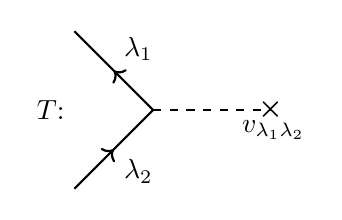
\begin{tikzpicture}

	\draw[thick, ->- = 0.5] (0,0) -- (1,1);
	\draw[thick, ->- = 0.5] (1, 1) -- (0,2);
	\draw[thick, dashed] (1, 1) -- (2.5, 1);
	\node[thick] at (2.5,1){$\cross$};
	\node[anchor = north west, thick] at (0.5, 0.5) {$\lambda_2$};
	\node[anchor = south west, thick] at (0.5, 1.5) {$\lambda_1$};
	\node[anchor = north west, thick] at (2, 1) {$v_{\lambda_1\lambda_2}$};
	\node[anchor = east] at (0, 1) {$T$:};
\end{tikzpicture}
\caption{Scattering from an external potential $v_{\mu\nu}c_{\mu}^\dagger c_{\nu}$}
\end{figure}


\begin{figure}
\centering
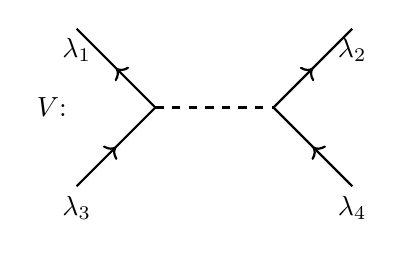
\begin{tikzpicture}

	\draw[thick, ->- = 0.5] (0,0) -- (1,1);
	\draw[thick, ->- = 0.5] (1, 1) -- (0,2);
	\draw[thick, dashed] (1, 1) -- (2.5, 1);
	\draw[thick, ->- = 0.5] (3.5, 0) -- (2.5, 1);
	\draw[thick, ->- = 0.5] (2.5, 1) -- (3.5, 2);
	
	\node[anchor = north] at (0, 0){$\lambda_3$};
	
	\node[anchor = north] at (0, 2){$\lambda_1$};	
	
	\node[anchor = north] at (3.5, 0){$\lambda_4$};

	\node[anchor = north] at (3.5, 2){$\lambda_2$};
	
	\node[anchor = east] at (0, 1) {$V$:};
\end{tikzpicture}
\caption{Exchange interaction between two particles.}
\end{figure}


\section{Coherent states for bosons}

\section{Grassman variable}
\section{Koherente tilstander for fermioner}







\end{document}